\documentclass[a4paper]{BACE}
\usepackage{pdflscape}
\usepackage{longtable}
\usepackage{xargs,xspace}
\usepackage{caption,subcaption,tabulary,multirow,bigdelim}
\usepackage{soul} %Do wywalenia!!!
\usepackage[colorinlistoftodos,prependcaption,textsize=tiny,textwidth=2.8cm]{todonotes}
\newcommandx{\odp}[2][1=]{\todo[linecolor=red,backgroundcolor=red!25,bordercolor=red,#1]{#2}}

\interfootnotelinepenalty=10000

\newcommand{\MCcube}{MC$^3$\xspace}
\newcommand{\gretlcmd}[1]{\lstinline!#1!\xspace}
\newcommand{\gretlcmdf}[1]{\inline{#1}\xspace}
\newcommand{\baceopts}[1]{\vspace*{10pt}\noindent\gretlcmd{#1}}
\makeatletter
\@mparswitchfalse%
\makeatother

\begin{document}
	\pagestyle{headings}
	\maketitle
	
	\begin{abstract}
		This paper presents a software package called \pkg{BACE}
		(Bayesian Averaging of Classical Estimates) which offers model-building strategy
		for various limited dependent variable models,
		including logit and probit models, ordered logit and probit
		models, multinomial logistic regression, Poisson regression, Tobit model, and interval regression.
		\pkg{BACE} strategy is a model selection method that incorporates both classical estimation and Bayesian techniques. 
		It solves the problem of computation speed and model uncertainty that arise when dealing with a large number of competing advanced statistical models.
		Our \pkg{BACE}
		package is both  fast and capable of delivering consistent results.
		The package  also provides implementation of the latest proposals
		of BIC variants,
		and the latest measures of jointness. We use \pkg{gretl}
		(GNU Regression, Econometrics, and Time-series Library),
		a popular, free, and open-source software for econometric
		analysis that features an easy-to-use graphical user interface (GUI).
	\end{abstract}
%	\jelcodes{C11, C21, C51}
	
	\section*{Project's main page:}
	\begin{quote}
		\centering	
		\url{https://sourceforge.net/projects/bace-for-gretl}
	\end{quote}
	
	\tableofcontents
	
	\section*{Changelog}
	\begin{description}
		\item[1.3] Massive changes and improvements:
		\begin{itemize}[label={--}]
			\item Extra package speed-up.
			\item New estimators added: logit (including ordered
				and multinomial), probit (including ordered),
				tobit, poisson, and intreg.
			\item Fixed bug in checking collinearity of
				independent variables -- now correct estimator
				is used instead of hardwired OLS.
			\item Correct model priors for truncated distributions.
			\item New MC3 strategy: taken directly from BMA package.
			\item New jointness measures.
			\item New \texttt{BACE()} bundle-based interface (default).
			\item Fix bug in \texttt{BACE\_GUI()} in constant type
				selection and general reorganization of GUI interface.
			\item Fixed bug when "can be dropped" option is used.
			\item New model types.
			\item Updated docs.
			\item Adding possibility for centering or standardizing variables.
			\item New BIC versions.
			\item Graphs added.
			\item Overloading parameters in options bundle.
			\item Clean up the code.
		\end{itemize}	
		\item[1.2] Several changes:
		\begin{itemize}[label={--}]
			\item Some typos in output.
			\item Getting rid of calls to deprecated functions.
			\item New jointness measures.
		\end{itemize}
		\item[1.1] Several changes:
		\begin{itemize}[label={--}]
			\item Documentation in PDF.
			\item Fix of several issues and bugs for model with only one
			explanatory variable and without constant.
			\item Change the option of the constant type from "random"
				to "can be dropped".
		\end{itemize}
		\item[1.0] Initial version.
	\end{description}

	\section*{To do}
	\begin{itemize}
		\item Simplify "if" condition for Y lags in \texttt{BACE\_estimate()}.
		\item Simplify \texttt{BACE\_initial\_model()}.
	\end{itemize}
	
	\section{Introduction}
In article \cite{SalaMartinDoppelhoferMiller_BACE} authors suggest a
technique for averaging the parameter estimates -- Bayesian Averaging
of Classical Estimates (BACE), which enables to measure the importance of
particular potential regressors. This approach is alternative to the
familiar and earlier-applied Bayesian Model Averaging (BMA) technique,
from which it differs mainly because of its less restrictive \textit{prior}
assumptions. The authors showed that BACE weighting method may
be understood as a limiting case of BMA approach  when the \textit{prior}
information is dominated by the data. The averaging of the parameter
estimates is performed across all possible combinations of linear regression models
obtained by means of Ordinary Least Squares (OLS)
 with classical assumptions.

The BACE approach has several interesting features in relation to
the techniques such as BMA or robustness-checking methods (\textcolor{red}{reference}).
First of all, it is not necessary to make assumptions concerning
\textit{prior} distribution for parameters but only
one simple assumption, on the expected model size.

An example of the application of the BACE technique for forecasting
macroeconomic indicators can be found, among others, in the articles
\cite{vanDijk2004Forecasting, AlbisMapa2014MPRA55902, BialowolskiKuszewskiWitkowski2015Empirica}.
	\section{Methodological background}\label{sec:Method_back}
\subsection{Model averaging and marginal data density approximation}\label{MA_basics}
As we know, probability can be used to describe the degree
of belief associated with different specifications when
comparing them using the Bayesian approach. For example,
based on posterior probability, we can quickly compare two
mutually exclusive (non-nested) and jointly exhaustive models
with various subsets of variables. Hence, the posterior odds
ratio for a model $M_l$ versus model $M_n$ can be obtained
using the following formula:
\begin{equation}
	\frac{\Prob(M_l \mid y)}{\Prob(M_n \mid y)}=\frac{\Prob(M_l)}{\Prob(M_n)}\frac{p(y \mid M_l)}{p(y \mid M_n)},
	\label{eq:posterior_odds_ratio}
\end{equation}
where $\frac{\Prob(M_l)}{\Prob(M_n)}$ is the prior odds ratio,
$\frac{p(y \mid M_l)}{p(y \mid M_n)}$ is the Bayes factor,
$p(y \mid M_l)$ and $p(y \mid M_n)$ are marginal data densities. 

If the posterior ratio $\frac{\Prob(M_l \mid y)}{\Prob(M_n \mid y)}$
is greater than one, it indicates that the data supports
model $M_l$ over model $M_n$.

As we can easily see, the key element needed to calculate
the Bayes factor is the normalizing constant, which is given
by the equation:
\begin{equation}
	p(y \mid M_r)=\int p(y \mid \theta_r, M_r)p(\theta_r \mid M_r)d\theta_r,
	\label{eq: p_y}
\end{equation}
where $\theta_r$ is the vector of unknown parameters,
$p(y|\theta_r, M_r)$ can be interpreted as likelihood function
under model $M_r$, and $p(\theta_r|M_r)$ is a prior
distribution of the parameters $\theta_r$.

In some relatively simple models, such as linear regression, the marginal
data density can be represented by a closed-form analytic
expression \citep[][]{zellner1971, fernandezleysteel2001b, koop2003}.
However, in many situations, even though it is a simple concept,
the marginal data density is difficult to calculate, especially
in high-dimensional models where numerical integration is more
computationally demanding
\citep[see][]{Newton_Raftery_1994, gelman2013bayesian, Pajor2017}.
This is particularly problematic in model averaging, where we
can have a large number of possible explanatory variables $(K)$
and therefore many potential combinations $(2^K)$ to calculate
in a relatively short time. For this reason, one possible
solution to overcome this problem is to use an approximation
of the integral in Equation \ref{eq: p_y} by Schwarz criterion
\citep{Schwarz_1978}. The \pkg{BACE} method with Schwarz
criterion refers to this solution by conducting a fast algorithm
of model averaging with a reasonably accurate marginal data
density approximation. Additionally, it is worth noting that
the \pkg{BACE} method also provides a good approximation of
estimated characteristics  and it is capable of replicating
the complex reduction strategy \citep{Kufel_jae_2020}.

In our \pkg{BACE} package, we use the latest approximations
of $p(y \mid M_r)$, which are popular in the frequentist
approach, and we briefly present them further in this paper
\citep[][]{Raftery_1996, Bollen_2012, Bollen_2014, Peterson_2019, Bayarri_2019}: 
\begin{enumerate}
	\item Standard Bayesian information criterion (BIC)
		introduced by \cite{Schwarz_1978}, one of the most
		popular model selection  method, based on the following
		assumption:
		\begin{equation}
			\ln p(y \mid M_r) \approx \ln p(y \mid \hat \theta_r, M_r) - \frac{k_r}{2}\ln N,
			\label{eq: BIC}
		\end{equation}
		where $\hat \theta_k$ is maximum likelihood estimator of
		parameters $\theta_k$, $k_r$ is a number of estimated
		parameters within the model $M_r$ and $N$ is the number
		of observations.
    \item Haughton’s BIC (HBIC) -- variant with additional retained
    	term of Taylor expansion of the $\ln p(y \mid M_k)$
    	around the MLE estimator \citep[][]{Haughton_1988, KassRaftery-BayesFactors-1995}:
	    \begin{equation}
	    	\ln p(y \mid M_r) \approx \ln p(y \mid \hat \theta_r, M_r) - \frac{k_r}{2}\ln N + \frac{k_r}{2}\ln (2\pi).
	    \end{equation}
	\item The Information Matrix-Based BIC (IBIC) proposed by
		\cite{Bollen_2012}, which includes another part of the
		Taylor expansion, this time Fisher information matrix
		$I(\hat \theta)$ evaluated at $\hat \theta$:
		\begin{equation}
			\ln p(y \mid M_r) \approx \ln p(y \mid \hat \theta_r, M_r) - \frac{k_r}{2}\ln N + \frac{k_r}{2}\ln (2\pi) -\frac{1}{2}\ln \left| I(\hat \theta) \right|.
			\label{eq: IBIC}
		\end{equation}
	\item Extended Bayesian Information Criteria (EBIC)
		introduced by \cite{Chen_Chen_2008} -- standard BIC
		with additional expression  that penalizes a model
		based on the number of candidate models of the same size:
		\begin{equation}
			\text{EBIC} = \text{BIC} - \gamma \ln \binom{K}{k_r}.
			\label{eq: EBIC}
		\end{equation}
\end{enumerate}

Using \pkg{BACE}, we can also easily evaluate the mean and
variance of the parameters $\theta$ across the entire model
space \citep[][]{Leamer1978}:

\begin{align}
	\E(\theta \mid y) &\approx \sum_{r=1}^{2^K}\Prob(M_r\mid y)\E(\theta_r \mid y,M_r),\\\nonumber
	\VAR(\theta \mid y) &\approx 
	\sum_{r=1}^{2^K}\Prob(M_r \mid y)\VAR(\theta_r  \mid y,M_r) +\\
	&+ \sum_{r=1}^{2^K}\Prob(M_r \mid y) \left(\E(\theta_r \mid y, M_r) - \E(\theta \mid y)\right)^2,
\end{align}
where $\E(\theta_r \mid y,M_r)$ and $\VAR(\theta_r \mid y,M_r)$
are the OLS (or MLE) estimates of $\theta_r$
from model $M_r$ and $2^K$ denotes total model space.

Following \cite{Ley_Steel_jae_2009}, let us assume that
each regressor enters a model independently of the others
with a prior probability $\psi \in [0, 1]$ (the prior
probability of inclusion). We offer two options here:
either the user provides a $\psi$ vector with individual
prior inclusion probabilities for each variable manually
(see \gretlcmd{Options["psi"]} on page~\pageref{opts:psi}),
or we use the theoretical prior model size $(W)$ distribution.
In our \pkg{BACE} package, we provide two popular variants
of such distributions \citep[see][]{Ley_Steel_jae_2009,steel2011}:
\begin{itemize}
	\item Binomial~\citep{Forsyth_2018}:
		\begin{equation}
			\Prob(W=k_r) = \binom{K}{k_r}\Prob(M_r),
			\label{eq:prior_model_size_binomial}
		\end{equation}
		with corresponding prior model probabilities as 
		\begin{equation}
			\Prob(M_r)=\psi^{k_r}(1-\psi)^{K-k_r},
			\label{eq:prior_model_probs_binomial}
		\end{equation}
		and expected model size $\E(W) = K\psi$;
	\item Beta-binomial~\citep{wakefield2013bayesian}:
		\begin{equation}
			\Prob(W=k_r) = \binom{K}{k_r}\Prob(M_r),
			\label{eq:prior_model_size_binomial-beta}
		\end{equation}
		where we assume that $\psi$ follows a Beta
		distribution with hyperparameters $a$ and $b$, both
		of which are greater than zero. This results in the
		following corresponding prior model probabilities%
		\footnote{The reason why we use the gamma function
			here instead of the beta function is that
			\pkg{gretl} provides the former but not the latter.}:
		\begin{equation}
			\Prob(M_r) = \frac{\Gamma (K+1)}{\Gamma(k_r+1)\Gamma(K-k_r+1)}\cdot
			\frac{\Gamma(a+k_r)\Gamma(K+b-k_r)}{\Gamma(a+b+k_r)} \cdot \frac{\Gamma(a+b)}{\Gamma(a)\Gamma(b)}
			\label{eq:prior_model_probs_binomial-beta}
		\end{equation}
		with expected model size $\E(W) = K\frac{a}{a+b}$.
		Furthermore, following \cite{Ley_Steel_jae_2009},
		we use $a = 1$ as dafault setting.
\end{itemize}

We assume that the user can specify just one hyperparameter
for the model prior, i.e., the expected model size
$\E(W) = W^\star \in(0,K)$\label{eq:W_star_definition}.
Our \pkg{BACE} package will automatically calculate the
prior probabilities for all competitive models. This is
a very convenient and flexible solution, similar to
approaches known from \cite{fernandezleysteel2001b}
and \cite{SalaMartinDoppelhoferMiller_BACE}.

In the case of a Binomial prior, if we specify
$W^\star = \frac{K}{2}$, which is the average number of
potential independent variables, then we have $\psi = 0.5$,
and thus, the prior model probability distribution is uniform.
An example for $K = 7$ is shown in Figure~\ref{fig:model_priors:subfig:uniform},
together with the corresponding prior model size distribution
shown in Figure~\ref{fig:model_priors:subfig:uniform-size}.

In the case of a Beta-binomial prior, if we specify
$W^\star = \frac{K}{2}$, then we have $b = 1$, which results
in a uniform prior distribution for the model size. An
example for $K = 7$ is shown in
Figure~\ref{fig:model_priors:subfig:beta-binomial-size},
together with the corresponding prior model probabilities
shown in Figure~\ref{fig:model_priors:subfig:beta-binomial}.

\begin{figure}[h!]
	\centering
	\begin{subfigure}[b]{0.24\textwidth}
		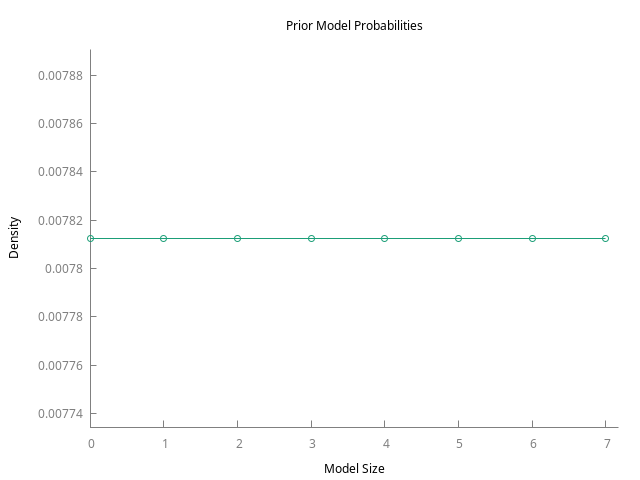
\includegraphics[width=1\textwidth]{PNG/ModelPriorDist_uniform}
		\caption{}
		\label{fig:model_priors:subfig:uniform}
	\end{subfigure}
	\begin{subfigure}[b]{0.24\textwidth}
		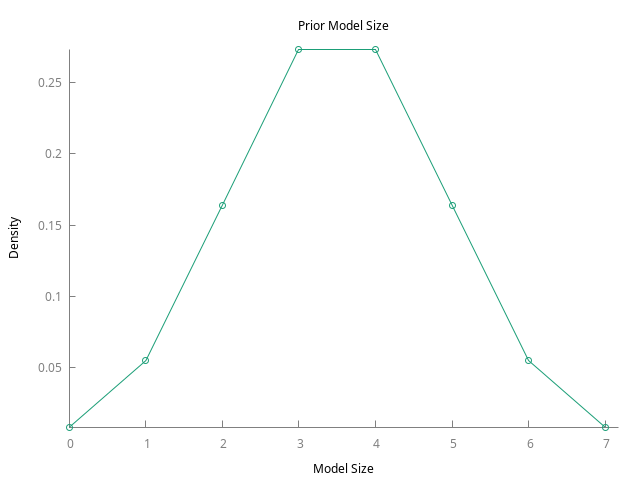
\includegraphics[width=1\textwidth]{PNG/ModelSizePriorDist_uniform}
		\caption{}
		\label{fig:model_priors:subfig:uniform-size}
	\end{subfigure}
	\begin{subfigure}[b]{0.24\textwidth}
		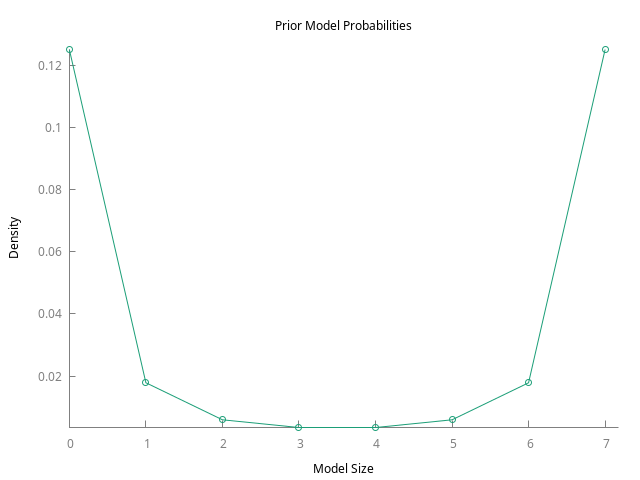
\includegraphics[width=1\textwidth]{PNG/ModelPriorDist_beta-binomial}
		\caption{}
		\label{fig:model_priors:subfig:beta-binomial}
	\end{subfigure}
	\begin{subfigure}[b]{0.24\textwidth}
		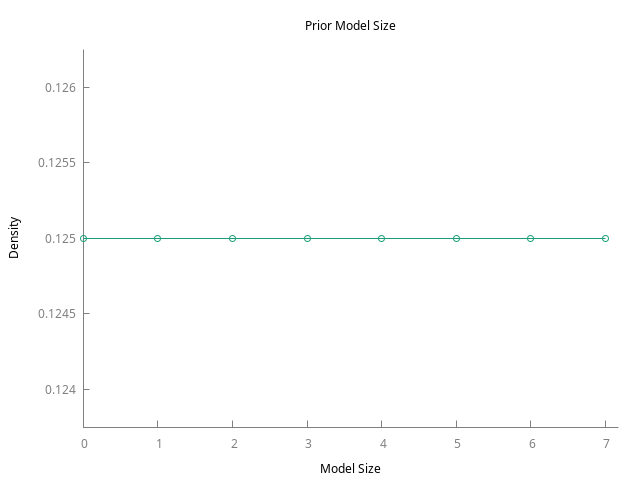
\includegraphics[width=1\textwidth]{PNG/ModelSizePriorDist_beta-binomial}
		\caption{}
		\label{fig:model_priors:subfig:beta-binomial-size}
	\end{subfigure}
	\caption{Prior model probabilities with associated prior
		model size for $K=7$ and $W^\star=\frac{K}{2}$,
		when model includes constant term}
\end{figure}

Sometimes, in a regression model, we do not include a constant
term \citep[see][]{KrolzigHendry-Computer_automation-2001,Kufel_jae_2020}.
This modelling strategy means that the model space is reduced
to $2^{K-1}$ possible combinations by excluding one specification
that consists of only a constant term, i.e., a model with no
explanatory variables. As a consequence, we should reflect
this in the \pkg{BACE} modeling by using a truncated prior
model size distribution.

From the definition of conditional probability, we can
define the density of a truncated random variable as
\cite[see][pp~864]{greene_econometric_a}:
\begin{equation}
	f\left(x | x > a\right) = \frac{f(x)}{\Prob(x > a)} .
\end{equation}
Because in our package, we assume that the user defines only
the expected model size $\E(W) = W^\star$, we have to rescale
the prior model size distribution so that it sums up to 1 and
has an expected value equal to $W^\star$. To do this, we have
to find the root of the following equation
\citep[see][]{Atwood1980,TripathiGuptaGurland-Estimation-1994}:
\begin{equation}
	\frac{\E(W)}{1-\Prob(W=0)} - W^\star = 0.
	\label{eq:solve_for_truncated_dist}
\end{equation}
We solve Equation~(\ref{eq:solve_for_truncated_dist})
numerically using \pkg{gretl}'s built-in \gretlcmd{fzero}
function. Note that for edge cases, i.e., when
$W^\star\approx 0$ or $W^\star\approx K$, the solution to
Equation~(\ref{eq:solve_for_truncated_dist}) may not exist.
Examples for $K=7$ are shown in
Figures~\ref{fig:model_priors:subfig:uniform-TR}-%
\ref{fig:model_priors:subfig:beta-binomial-size-TR}.

\begin{figure}[h!]
	\centering
	\begin{subfigure}[b]{0.24\textwidth}
		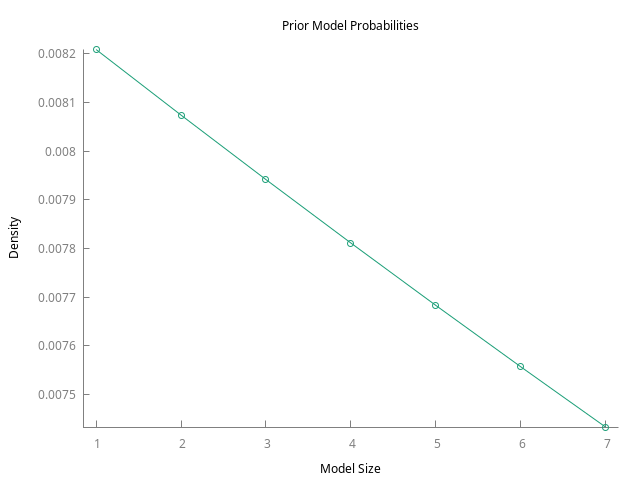
\includegraphics[width=1\textwidth]{PNG/ModelPriorDist_uniform-TR}
		\caption{}
		\label{fig:model_priors:subfig:uniform-TR}
	\end{subfigure}
	\begin{subfigure}[b]{0.24\textwidth}
		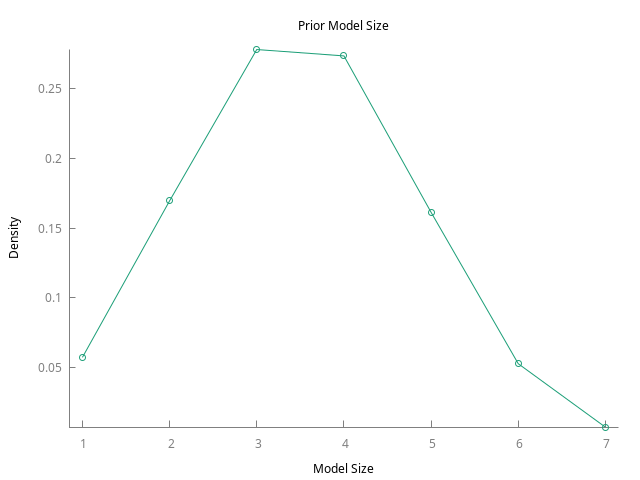
\includegraphics[width=1\textwidth]{PNG/ModelSizePriorDist_uniform-TR}
		\caption{}
		\label{fig:model_priors:subfig:uniform-size-TR}
	\end{subfigure}
	\begin{subfigure}[b]{0.24\textwidth}
		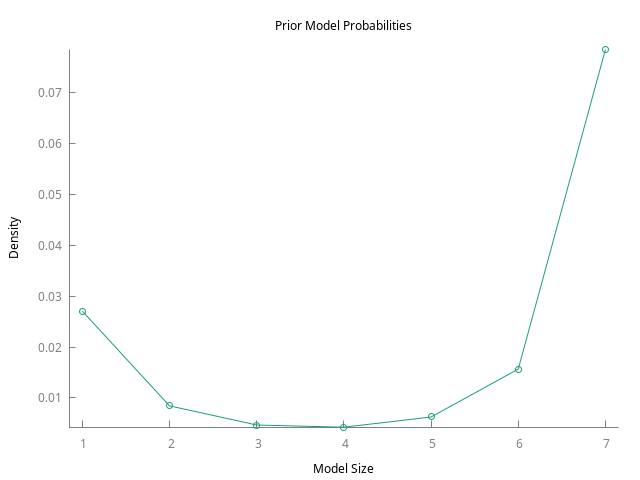
\includegraphics[width=1\textwidth]{PNG/ModelPriorDist_beta-binomial-TR}
		\caption{}
		\label{fig:model_priors:subfig:beta-binomial-TR}
	\end{subfigure}
	\begin{subfigure}[b]{0.24\textwidth}
		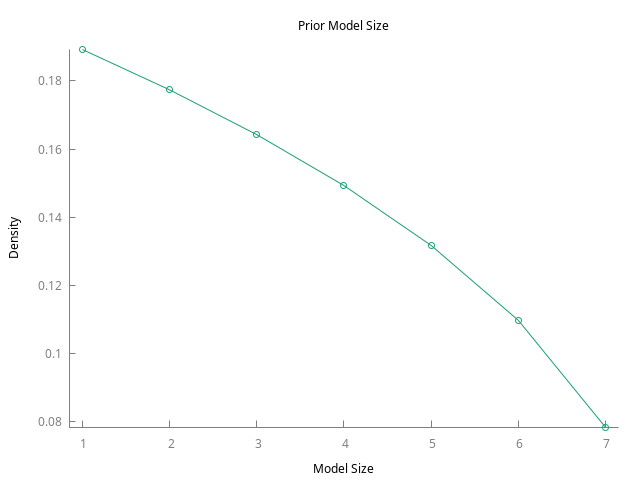
\includegraphics[width=1\textwidth]{PNG/ModelSizePriorDist_beta-binomial-TR}
		\caption{}
		\label{fig:model_priors:subfig:beta-binomial-size-TR}
	\end{subfigure}
	\caption{Prior model probabilities with associated prior
	model size for $K=7$ and $W^\star=\frac{K}{2}$,
		when model does not include a constant term}
\end{figure}

On the basis of Bayes' formula, the posterior probability
of any model $M_j$ can be computed as follows:
\begin{equation}
	\Prob(M_j|y) = \frac{\Prob(M_j)p\left( y \mid M_j\right)}
	{\sum_{r=1}^{2^K}\Prob(M_r)p\left( y \mid M_r\right)}
	\label{eq: model_avg}
\end{equation}
It is easy to see that Equation \ref{eq: model_avg} allows
us to calculate the probability for each model $M_r$ using
corresponding prior probabilities $\Prob\left( M_r\right)$ and
the density of the marginal distribution $p(y \mid M_j)$,
here approximated by expressions \ref{eq: BIC} -- \ref{eq: IBIC}.

Another useful characteristic popular in the model averaging
approach is the Posterior Inclusion Probability (PIP), which
is defined as the posterior probability that the independent
variable $x_i$ is relevant in explaining the dependent variable
(\cite{Leamer1978, mitchell_beauchamp_1988}). In our case, the
PIP is calculated using Monte Carlo integration, as the sum of
the posterior model probabilities for all models that include
the specific independent variable \citep{Forte_Garcia_Steel_2018}.

Although posterior characteristics are often of interest,
predicting future values of the dependent variable can be
valuable in many cases. With the \pkg{BACE} approach, we can
also perform predictive inference across the entire model space.
If we have the matrix $X_r^*$ containing explanatory variables
for each of the out-of-sample data points, we can use a
weighted average of the individual model forecasts to make
predictions about unobserved values of the dependent variable.

To determine the significance of determinants and the most
likely models across the model space, we utilize the \MCcube
sampling algorithm, which was originally developed by
\cite{madiganyork1995}. The \MCcube algorithm is one of the most
widely used MCMC algorithms in many statistical packages for
model averaging, for example:
\cite{LamnisosGriffinSteel2013,JSSv068i04,rafteryhoetingvolinskypainteryeung_bma,JSSv104i02}.

	\subsection{The limited  dependent variable models}
In many practical applications, it is common to encounter
phenomena with discrete or censored dependent variables.
Our \pkg{BACE} package includes several models that can
handle this issue, including the most popular ones such
as logit and probit models, as well as their ordered
specifications and multinomial logistic regression.
Additionally, the package provides support for Poisson
regression, Tobit model, and interval regression%
\footnote{The \pkg{BACE} package also includes linear
	regression models. However, since the dependent variable
	is not bounded in these models, linear regression is
	not the main focus of our interest.}.
In all of these cases, the dependent variable is either
dichotomous (i.e., taking the values zero or one),
categorical, a count, or censored.
In the remainder of this subsection, we present the standard
and popular models for limited dependent variable included
in our \pkg{BACE} package, which are also discussed in
\cite{koop2007bayesian, hosmer:logistic, Winkelmann_2008, verbeek2018guide}
and \cite{cottrell_luchcetti_gretl_manual}.

First, let us analyze the logit and probit models. The logit
and probit models are two types of regression models commonly
used to predict a binary dependent variable. Logit models are
based on the logistic distribution, while probit models are
based on the normal distribution. Let us consider a model of the form:
\begin{equation}
	z_i= \sum_{j=1}^{k_r}x_{ij}\beta_{j} + \epsilon_i, 
\end{equation}
and	
\begin{equation*}	
	y_i= \left \{\begin{array}{ll}
					1 & \text{if } z_i >0 \\
					0 & \text{if } z_i \leq 0,
				\end{array}\right.
\end{equation*}
where $z_i$, $i=1, \dots, N$ is an unobserved variable, while
$y_i$ is binary, observed data. $x_{ij}$ and $\beta_j$ are
explanatory variables and regression coefficients in model
$M_r$ for $j=1,\dots, k_r$.
If $\epsilon_i \overset{\text{iid}}{\sim} N(0, 1)$, then we
have a probit model. Otherwise, we obtain a logit regression.

In the next step, let us specify logit and probit models, where
we consider the choice between $L$ alternatives, numbered from 1 to $L$:
\begin{equation}
		z_i= \sum_{j=1}^{k_r}x_{ij}\beta_{j} + \epsilon_i,
%		z_i= x_{ri}\beta_{ri} + \epsilon_i, 
\end{equation}
and
\begin{equation*}
		y_i= \left \{ 
			\begin{array}{lc}
					 1 & \text{if } \alpha_0 < z_i \leq  \alpha_1 \\
					 2 & \text{if } \alpha_1 < z_i \leq  \alpha_2 \\
					 \vdots & \vdots \\
					L & \text{if } \alpha_{L-1} < z_i \leq  \alpha_{L}, \\
			\end{array}\right.
\end{equation*}
where unknown $\alpha_i$s are cutpoints with
$\alpha_0 = -\infty, \alpha_1 = 0$ and $\alpha_L = \infty$.
Assuming that $\epsilon_i$ is iid and standard normal, we obtain
the ordered probit model, whereas the logistic distribution
gives the ordered logit model.

The latest considered model of this kind is multinomial logistic
regression. It is an extension of logistic regression modeling
for cases where the dependent variable is not binary but can
take the values $0,1, \ldots, p$ and the categories are nominal,
meaning they do not have a natural order.

The model can be written in the following form:
\begin{align}
	\Prob\left(y_i= k\mid x_i\right) &= \frac{\exp \left( x_i\beta_k\right)} {1+\sum_{j=1}^{p}\exp{(x_i\beta_j)}}, k > 0,\\
	\Prob\left(y_i= 0\mid x_i\right) &= \frac{1} {1+\sum_{j=1}^{p}\exp{(x_i\beta_j)}}.
\end{align}

Poisson regression is a model used to predict count data
occurrences. That is, a dependent variable $y$ takes values
$k=0,1, 2\ldots$ from the Poisson distribution. Under this
assumption, the probability of the outcome variable $y$
conditional upon regressors is given by:
\begin{equation}
	\Prob\left(y_i= k\mid x_i\right)  = \frac{\exp \left\{-\lambda_{i} \right\} \lambda_{i}^k}{k!},
\end{equation}
where $\lambda_i= \exp(\sum_{j=1}^{k_r}x_{ij}\beta_{j})$ in model $M_r$.

The Tobit model is a type of regression model used to analyze
censored data, which refers to data with a lower or upper bound
on the dependent variable. Consider the following Tobit model
(type I) with two thresholds \citep{cottrell_luchcetti_gretl_manual}:
\begin{equation}
	z_i= \sum_{j=1}^{k_r}x_{ij}\beta_{j} + \epsilon_i,
	\label{eq: unobs_dep}
\end{equation}
and
\begin{equation}
	y_i= \left \{ 
	\begin{array}{ll}
		a & \text{for }  z_i \le a\\
		z_i &\text{for }  a < z_i < b\\
		b & \text{for }  z_i \ge b,\\
	\end{array}   \right.
\label{eq: tobit}
\end{equation}
where $\epsilon \sim N(0, \sigma^2)$. Usually the most
common specification is  $a=0$ and $b= \infty$.That is,
at zero, observations are censored from below, which means
that we do not observe any $z_i$ values that are negative \citep{verbeek2018guide}.

Another model that is available in the \pkg{BACE} package is
the interval regression. It is similar to the standard linear
regression, but it allows for the possibility of censoring
some data points due to measurement limitations or other
factors \citep{Stewart_1983, Bettin_Lucchetti_2012, cottrell_luchcetti_gretl_manual}.
In this case, we consider a data generating process with an
unobserved dependent variable $z_i$ (Equation \ref{eq: unobs_dep})
and an observed interval that contains this variable:
\begin{equation}
	m_i \leq z_i \leq  M_i.
\end{equation}
The interval can also be left-unbounded, i.e., $m_i = -\infty$
or right-unbounded, when $M_i = \infty$. In the case of
$m_i = M_i$, all observations are point observations and the
model reduces to a standard regression model, which is also
available in the \pkg{BACE} package. Please note that due to
the complexity of the censoring problem, the interval
regression model is only available in script form.

All of the mentioned models are available in the \pkg{BACE}
package. Through the use of model averaging analysis, it is
possible to estimate parameters, identify the key determinants,
and make predictions.

% BACE 3.2: interpretation and model averaging of ORs and AMEs.
\subsection{Model-averaged odds ratios and marginal effects}
\label{sec:or_ame_theory}
For binary and ordered response models, the regression coefficients
alone do not describe changes in outcome probabilities. The
\pkg{BACE} package therefore provides model-averaged odds ratios
(ORs) for binary and ordered logit models and average marginal
effects (AMEs) for binary and ordered logit and probit models.
Both quantities are first calculated within each model $M_r$ and
then averaged over the model space in the same way as the
parameter estimates in Section~\ref{MA_basics}. As there, the sums
over $2^K$ models are in practice approximated using the models
visited by the \MCcube algorithm.

We use the notation of the models described above. In model $M_r$
the latent variable is $z_i=x_i\beta+\epsilon_i=\sum_{j}x_{ij}\beta_j+\epsilon_i$,
where $x_{ij}$ is the $j$-th of $K$ candidate regressors and
$\beta_j=0$ whenever $x_j$ is not included in $M_r$. Let $F$ and $f$
denote the cumulative distribution function and the density of
$\epsilon_i$, i.e.\ the logistic ones for logit and the standard normal
ones for probit models. For a binary dependent variable
\begin{equation}
	\Prob(y_i=1\mid x_i,M_r)=F(x_i\beta)=1-\Prob(y_i=0\mid x_i,M_r),
	\label{eq:bace_prob_binary}
\end{equation}
and for an ordered one with $L$ categories and cutpoints
$\alpha_0=-\infty<\alpha_1<\dots<\alpha_L=\infty$
\begin{equation}
	\Prob(y_i=l\mid x_i,M_r)=F(\alpha_l-x_i\beta)-F(\alpha_{l-1}-x_i\beta),
	\quad l=1,\dots,L.
	\label{eq:bace_prob_ordered}
\end{equation}
Here $l$ indexes the observed outcome categories in increasing order;
their labels need not form a consecutive sequence.

\paragraph{Odds ratios for logit models.}
In the binary logit model the odds $\Prob(y_i=1\mid x_i,M_r)/\Prob(y_i=0\mid x_i,M_r)$
equal $\exp(x_i\beta)$, so a one-unit increase in $x_{ij}$ multiplies
the odds by $\mathrm{OR}_j=\exp(\beta_j)$. In the ordered logit model
(\ref{eq:bace_prob_ordered}), $\Prob(y_i\le l\mid x_i,M_r)=F(\alpha_l-x_i\beta)$,
so $\exp(\beta_j)$ is the common factor by which the odds
$\Prob(y_i>l\mid x_i,M_r)/\Prob(y_i\le l\mid x_i,M_r)$ change, the same
for every $l$. If $x_j\notin M_r$, then $\beta_j=0$ and $\mathrm{OR}_j=1$.

To take within-model coefficient uncertainty into account, we use the normal
approximation $\beta_j\mid y,M_r\ \dot{\sim}\ N\bigl(\E(\beta_j\mid y,M_r),\VAR(\beta_j\mid y,M_r)\bigr)$,
where $\E(\beta_j\mid y,M_r)$ and $\VAR(\beta_j\mid y,M_r)$ are the
MLE estimate and its estimated variance from model $M_r$. Then
$\mathrm{OR}_j$ is approximately lognormal and, for $x_j\in M_r$,
%\begin{align}
%	\E(\mathrm{OR}_j\mid y,M_r)&=\exp\!\Bigl(\E(\beta_j\mid y,M_r)+\tfrac12 \VAR(\beta_j\mid y,M_r)\Bigr),
%	\label{eq:bace_or_moment1}\\
%	\VAR(\mathrm{OR}_j\mid y,M_r)&=\Bigl[\exp\bigl(\VAR(\beta_j\mid y,M_r)\bigr)-1\Bigr]
%	\exp\!\Bigl(2\E(\beta_j\mid y,M_r)+\VAR(\beta_j\mid y,M_r)\Bigr),
%	\label{eq:bace_or_moment2}
%\end{align}
\begin{align}
	\E(\mathrm{OR}_j\mid y,M_r)&=\exp\!\Bigl(\E(\beta_j\mid y,M_r)+\tfrac12 \VAR(\beta_j\mid y,M_r)\Bigr),
	\label{eq:bace_or_moment1}\\
	\VAR(\mathrm{OR}_j\mid y,M_r)&=\Bigl[\exp\bigl(\VAR(\beta_j\mid y,M_r)\bigr)-1\Bigr]\nonumber\\
	&\quad\times\exp\!\Bigl(2\E(\beta_j\mid y,M_r)+\VAR(\beta_j\mid y,M_r)\Bigr),
	\label{eq:bace_or_moment2}
\end{align}
whereas for $x_j\notin M_r$ we have $\E(\mathrm{OR}_j\mid y,M_r)=1$ and
$\VAR(\mathrm{OR}_j\mid y,M_r)=0$. The model-averaged OR and its variance
are obtained analogously to $\E(\theta\mid y)$ and $\VAR(\theta\mid y)$:
\begin{align}
	\E(\mathrm{OR}_j\mid y)&\approx\sum_{r=1}^{2^K}\Prob(M_r\mid y)\,\E(\mathrm{OR}_j\mid y,M_r),\\
	\VAR(\mathrm{OR}_j\mid y)&\approx\sum_{r=1}^{2^K}\Prob(M_r\mid y)\,\VAR(\mathrm{OR}_j\mid y,M_r)\nonumber\\
	&\quad+\sum_{r=1}^{2^K}\Prob(M_r\mid y)\Bigl(\E(\mathrm{OR}_j\mid y,M_r)-\E(\mathrm{OR}_j\mid y)\Bigr)^2,
	\label{eq:bace_or_bma}
\end{align}
and the reported standard deviation is $\sqrt{\VAR(\mathrm{OR}_j\mid y)}$.
Thus, $\E(\mathrm{OR}_j\mid y)$ is \emph{not} simply the exponential of
the model-averaged coefficient $\E(\beta_j\mid y)$. In particular, an OR of one
corresponds to no change in odds, and the posterior mass of models
excluding a regressor contributes an OR of one. Exponentiating a
probit coefficient does not produce an odds ratio, so ORs are not
reported for probit models. These regressor-level ORs should not be
confused with the posterior \emph{model} odds ratios in
Equation~\ref{eq:posterior_odds_ratio}.

\paragraph{Average marginal effects.}
For a continuous regressor $x_j$, the average marginal effect on
the probability of category $l$ in model $M_r$ is
\begin{equation}
	\mathrm{AME}_{jl}(M_r)
	=\frac1{N}\sum_{i=1}^{N}
	\frac{\partial\Prob(y_i=l\mid x_i,M_r)}{\partial x_{ij}}.
	\label{eq:bace_ame_continuous}
\end{equation}
From (\ref{eq:bace_prob_binary}), in a binary logit or probit
\begin{equation}
	\frac{\partial\Prob(y_i=1\mid x_i,M_r)}{\partial x_{ij}}=\beta_j f(x_i\beta),
	\label{eq:bace_ame_binary}
\end{equation}
with the negative of this effect for $y_i=0$, and from
(\ref{eq:bace_prob_ordered}), in an ordered logit or probit
\begin{equation}
	\frac{\partial\Prob(y_i=l\mid x_i,M_r)}{\partial x_{ij}}
	=\beta_j\Bigl[f(\alpha_{l-1}-x_i\beta)-f(\alpha_l-x_i\beta)\Bigr],
	\label{eq:bace_ame_ordered}
\end{equation}
where the density at an infinite cutpoint ($\alpha_0$ or $\alpha_L$)
is zero.

For regressors taking only the values zero and one, the software
instead computes the average discrete change
\begin{equation}
	\mathrm{AME}_{jl}^{(0\to1)}(M_r)=\frac1{N}\sum_{i=1}^{N}
	\Bigl[\Prob(y_i=l\mid x_{ij}=1,x_{i,-j},M_r)
	-\Prob(y_i=l\mid x_{ij}=0,x_{i,-j},M_r)\Bigr],
	\label{eq:bace_ame_binary_regressor}
\end{equation}
where $x_{i,-j}$ denotes the remaining regressors, held at their observed
values. For a regressor absent from $M_r$, $\beta_j=0$ and all its marginal
effects are zero. Finally, the reported effects are averaged across models:
\begin{equation}
	\E(\mathrm{AME}_{jl}\mid y)\approx\sum_{r=1}^{2^K}\Prob(M_r\mid y)\,\mathrm{AME}_{jl}(M_r),
	\label{eq:bace_ame_bma}
\end{equation}
with $\mathrm{AME}_{jl}^{(0\to1)}(M_r)$ in place of $\mathrm{AME}_{jl}(M_r)$
for 0/1 regressors. The model-specific effects are evaluated at the
estimated coefficients $\E(\beta_j\mid y,M_r)$ and cutpoints; unlike
the OR variance (\ref{eq:bace_or_bma}), the procedure does not propagate
the within-model sampling variance and does not supply a standard deviation
of the AMEs. In every model and in the model average, the marginal effects
over the exhaustive outcome categories sum to zero (up to numerical
rounding), i.e.\ $\sum_{l}\E(\mathrm{AME}_{jl}\mid y)=0$. An effect of
$0.01$ corresponds to one percentage point.

Automatic recognition of 0/1 regressors requires both values to occur in
the estimation sample and is currently used only when no lagged dependent
variables have been introduced. Otherwise the program reports average
derivatives. For several dummy variables encoding one categorical regressor,
the 0-to-1 comparison is performed on each dummy separately; users should
interpret such changes with care, because a counterfactual holding the other
dummies fixed can represent an impossible combination of categories.
These are descriptive model-based effects, not causal effects without
additional identifying assumptions.

\subsection{Jointness measures}\label{sec:jointness_measures}
The main implementations of  model averaging are concerned
with the selection of variables when model uncertainty is
present. Another relevant issue which arises in this framework is to
identify whether different sets of two variables $x_i$ and $x_j$ are
substitutes, complements or neither over the model space. For that
reason, \cite{LeySteel2007} and \cite{DoppelhoferWeeks2009} define
ex-post jointness measures of dependence between different sets of
explanatory variables. Following \cite{Hofmarcher2018},
we can  use a general contingency Table \ref{tab:GeneralContingencyTable}
and easily calculate a number of jointness measures considered
in the literature. In \pkg{BACE} we have:

\begin{table}[h!tb]
	\centering
	\caption{General contingency table for two binary variables.}
	\begin{tabular}{l|ccc}\hline
		&\textit{B}	&	$\overline{B}$	&Total	\\\hline
		\textit{A}		&	a		&	b			& $a+b$		\\
		$\overline{A}$	&	c		&	d			& $c+d$		\\
		Total			&	$a+c$	&	$b+d$		& $a+b+c+d=N$\\\hline
	\end{tabular}
	\label{tab:GeneralContingencyTable}
\end{table}

\begin{itemize}\label{sec:jointess_numbers}
	\item The jointness measure $J_{\mathit{DW1}}$, first
		proposed in the \cite{DoppelhoferWeeks2005}:
		\begin{align}
			\begin{split}
				J_{\mathit{DW1}}(A,B) &  = \ln\left(\frac{\Prob(AB\mid y)}
				{\Prob(A\mid y) \Prob(B\mid y)}\right)\\
				& = \ln\left(\frac{aN}{(a+b)(a+c)}\right).
			\end{split}
			\label{DW_jointness1}
		\end{align}
	\item An alternative variant $J_{\mathit{DW2}}$ also
		proposed by \cite{DoppelhoferWeeks2009}:
		\begin{align}
			\begin{split}
				J_{\mathit{DW2}}(A,B) & =\ln\left(\frac {\Prob(AB \mid y)\Prob(\overline{A}\overline{B} \mid y)}
				{\Prob(A\overline{B}\mid y)\Prob(\overline{A}B\mid y)}\right) \\
				& = \ln\left(\frac{ad}{bc}\right).
			\end{split}
			\label{DW_jointness2}
		\end{align}
	\item The jointness statistics presented in \cite{LeySteel2007}:
		\begin{align}
			\begin{split}
				J_{\mathit{LS1}}(A,B) & = \frac{\Prob(AB\mid y)}{\Prob(A\mid y)+\Prob(B\mid y)-\Prob(AB\mid y)} \\
				& = \frac{a}{a+b+c}.
			\end{split}
			\label{LS_jointness1}
		\end{align}
	\item An additional variant of an earlier measure:
		\begin{align}
			\begin{split}
				J_{\mathit{LS2}}(A,B) & = \frac{\Prob(AB\mid y)}{\Prob(A\overline{B}\mid y)+\Prob(\overline{A}B\mid y)} \\
				& =  \frac{a}{b+c}.
			\end{split}
			\label{LS_jointness2}
		\end{align}
	\item The measure  proposed in \cite{Strachan2009}:
		\begin{align}
			\begin{split}
				J_{\mathit{St}}(A,B) & = \Prob(A\mid y)\Prob(B\mid y)
				\ln\left(\frac{\Prob(AB\mid y)}{\Prob(A\overline{B}\mid y)
					\Prob(\overline{A}B\mid y)}\right) \\
				& = \frac{a+b}{N}\frac{a+c}{N}\ln\left(\frac{aN}{bc}\right).
			\end{split}
			\label{St_jointness}
		\end{align}
	\item Yule's Q measure:
		\begin{align}
			\begin{split}
				J_{\mathit{YQ}}(A,B) & = \frac{\Prob(AB)\Prob(\overline{AB})-\Prob(A\overline{B})\Prob(\overline{A}B)}
				{\Prob(AB)\Prob(\overline{AB})+\Prob(A\overline{B})\Prob(\overline{A}B)} \\
				& = \frac{ad - bc}{ad + bc}.
			\end{split}
			\label{Yq_jointness}
		\end{align}
	\item The last  measure and also the default one,
		modified Yule's Q:
		\begin{equation}		
			J_{\mathit{YQ}} = \frac
			{\left(a+\frac{1}{2}\right)\left(d+\frac{1}{2}\right) -
				\left(b+\frac{1}{2}\right)\left(c+\frac{1}{2}\right)} 
			{\left(a+\frac{1}{2}\right)\left(d+\frac{1}{2}\right) +
				\left(b+\frac{1}{2}\right)\left(c+\frac{1}{2}\right) - \frac{1}{2}}.
			\label{YqM_jointness}
		\end{equation}
\end{itemize}

Information on the properties of these listed measures
and their interpretations can be found in the publication
of \cite{Hofmarcher2018}.

	\section{Implementation in \pkg{gretl}}\label{sec:BACE_implementation}
In this section, we describe the code of the \pkg{BACE}
package. First, we will characterize our code and the use
of both: the command line and the GUI interfaces, then we
will present some examples of using the \pkg{BACE}.
Finally, we will show the outputs that are returned.

\subsection{The core of the \pkg{BACE} code}
The \pkg{BACE} package consists of 4 public and 14
private functions. The name of each function starts
with the \cmd{BACE\_} prefix. The public functions are:
\begin{enumerate}
	\item \cmd{BACE()}~see~\ref{sec:BACE()}
	\item \cmd{BACE\_GUI()}~see~\ref{sec:BACE_GUI()}
	\item \cmd{BACE\_Print()}~see~\ref{sec:BACE_Print()}
	\item \cmd{BACE\_Plot()}~see~\ref{sec:BACE_Plot()}
\end{enumerate}

\subsubsection{\cmd{BACE()}}\label{sec:BACE()}
This is a core package function which runs and controls
the main loop. As a consequence, it is a prime interface
to the \pkg{BACE} package. The \cmd{BACE()} function
returns a bundle with all information needed to print
and/or plot results anytime. One can print the results
by calling \cmd{BACE\_Print()} or plot graphs by calling
\cmd{BACE\_Plot()}. The signature of \cmd{BACE()}
function is as follows:
\begin{lstlisting}
function bundle BACE (series Y "Dependent variable",
  list X_list "List of indenpendent variables (X)",
  bundle Options[null])	
\end{lstlisting}
The first two options are mandatory, while the last one
is an optional collection of additional arguments. Those
arguments are defined with the following default values:\label{sec:default_option_bundle}
\begin{lstlisting}
scalar Options["Y_AR_p"] = 0
scalar Options["with_const"] = 1
scalar Options["model_prior"] = 2
scalar Options["avg_model_size"] = avg_model_size_tmp
scalar Options["alpha"] = 0.6
scalar Options["Nrank"] = xmin(2^(k+Y_AR_p_tmp-1), 40)
scalar Options["do_joint"] = 0
scalar Options["Npredict"] = 0
scalar Options["Nrep"] = Nrep
scalar Options["burn"] = 10
scalar Options["verbosity"] = 2
scalar Options["show_progress"] = do_show_progress
scalar Options["do_plot"] = do_plot_tmp
string Options["model_type"] = "linear"
scalar Options["data_trans"] = 0
scalar Options["bic_type"] = 1
scalar Options["hyperparameter"] = 0.5 # gamma for EBIC
scalar Options["binary_threshold"] = 0.5
scalar Options["low"] = 0
scalar Options["high"] = NA
scalar Options["_gui"] = 0	
\end{lstlisting}
where \textit{k} stands for the number of independent variables,
\lstinline!scalar avg_model_size! is calculated according to
the following formula:
\begin{equation}
	\texttt{\lstinline!avg\_model\_size!} = \left\{
	\begin{array}{lll}
		\textrm{\lstinline!(k + Y\_AR\_p\_tmp)/2!} & \mathrm{if} & \textrm{\lstinline!with_const \!= 2!},\\
		\textrm{\lstinline!(k + Y\_AR\_p\_tmp + 1)/2!} & \mathrm{elsewhere}, &\\
	\end{array}
	\right.
	\label{eq:avg_model_size_setup}
\end{equation}
\lstinline!scalar Nrep! takes the following values:
\begin{equation}
	\texttt{\lstinline!Nrep!} = \left\{
	\begin{array}{ccl}
		10^4 & \mathrm{if} & k \leq 15,\\
		10^5 & \mathrm{if} & k \in [16;19],\\
		10^6 & \mathrm{if} & k \geq 20,\\
	\end{array}
	\right.
	\label{eq:Nrep_setup}
\end{equation}
\lstinline!scalar show_progress! takes the following values:
\begin{equation}
	\texttt{\lstinline!show\_progress!} = \left\{
	\begin{array}{cll}
		1 & \mathrm{if} & \textrm{\lstinline!$sysinfo!\texttt{\small.gui\_mode}},\\
		0 & \mathrm{elsewhere}, &\\
	\end{array}
	\right.
	\label{eq:show_progress_setup}
\end{equation}
and \lstinline!scalar do_plot! takes the following values:
\begin{equation}
	\texttt{\lstinline!do\_plot!} = \left\{
	\begin{array}{cll}
		1 & \mathrm{if} & \textrm{\lstinline!$sysinfo!\texttt{\small.gui\_mode}},\\
		0 & \mathrm{elsewhere}. &\\
	\end{array}
	\right.
	\label{eq:do_plot_setup}
\end{equation}
Most of the optional parameters listed above are of
numerical type and they may be gathered into following
groups according to what kind of numbers they can take%
\footnote{Note, that the \lstinline!scalar _gui! is
	for internal use only and must not be modified
	by user at any rate.}:
\begin{enumerate}
	\item Integers: \lstinline!Y_AR_p!, \lstinline!with_const!,
	\lstinline!model_prior!, \lstinline!Nrank!, \lstinline!do_joint!,
	\lstinline!Npredict!, \lstinline!Nrep!, \lstinline!burn!,
	\lstinline!verbosity!, \lstinline!data_trans!, \lstinline!bic_type!.
	\item Booleans: \lstinline!show_progress!, \lstinline!do_plot!.
	\item Scalars: \lstinline!avg_model_size!, \lstinline!alpha!,
	\lstinline!binary_threshold!.
\end{enumerate}
Optional parameters control the following package options:
\begin{enumerate}
	\item \textbf{Y\_AR\_p}: autoregression order of variable Y.
	\item \textbf{with\_const}: whether we include constant term
		in each estimated model?; possible values are: 0---without
		constant, 1---constant is always included, 2---constant
		may be dropped.
	\item \textbf{model\_prior}: model prior distribution to use;
		possible values are: 0---none, 1---Binomial, 2---Beta-Binomial.
	\item \textbf{avg\_model\_size}: expected average model size
		for model prior.
	\item \textbf{alpha}: significance level for the initial model.
	\item \textbf{Nrank}: number of top ranked models.
	\item \textbf{do\_joint}: do we perform jointness analysis?;
		possible values are: 0---none, 1---Doppelhofer-Weeks
		Measure (DW1), 2---Doppelhofer-Weeks Measure (DW2),
		3---Ley-Steel Measure (LS1), 4---Ley-Steel Measure (LS2),
		5---Strachan Measure, 6---Yule's Q Measure (YQ),
		7---Modified Yule's Q Measure (YQM).
	\item \textbf{Npredict}: number of out-of-sample forecasts.
		Note, that using this option makes \pkg{BACE} to perform
		an analysis on subsample.
	\item \textbf{Nrep}: total number of Monte Carlo iterations
		(model draws).
	\item \textbf{burn}: percentage of burn-in draws in \MCcube.
	\item \textbf{verbosity}: verbosity of the output: 1---basic
		results, 2---full results.
	\item \textbf{show\_progress}: do we show overall progress?
	\item \textbf{do\_plot}: do we produce graphs?
	\item \textbf{model\_type}: model type we should apply to
		the data; possible options are: 1---linear, 2---logit,
		3---probit, 4---poisson.
	\item \textbf{data\_trans}: shall the \pkg{BACE} transform
		data before analysis?; possible options are: 0---none,
		1---centering, 2---standarizing.
	\item \textbf{bic\_type}: Bayesian information criterion
		version which should be used; possible values are:
		1---bic, 2---hbic, 3---ibic, 4---ebic.
	\item \textbf{hyperparameter}: hyperparameter for prior
		setup; for now it is interpreted as $\gamma$ for ebic.
	\item \textbf{binary\_threshold}: applicable only for
		binary-dependent models; this value indicates the
		lowest probability for which $\hat{y}_i$ should take 1.
	\item \textbf{low}: applicable only for	\lstinline!tobit!
		model; this option controls tobit's \lstinline!--llimit!
		flag for setting left bound in censoring.
	\item \textbf{high}: applicable only for \lstinline!tobit!
		model; this option controls tobit's \lstinline!--rlimit!
		flag for setting right bound in censoring.
\end{enumerate}
Some of the above-mentioned parameters are over-loadable, which
means that their value may be passed either via an integer or
via string (case insensitive). Those parameters (together with
value-string mappings) are:\label{sec:over-loadable_options}
\begin{description}
	\item[\textbf{bic\_type}]: 'bic'=1, 'hbic'=2, 'ibic'=3, 'ebic'=4;
	\item[\textbf{model\_prior}]: 'none'=0, 'binomial'=1,
		'betabinomial'=2 (or 'beta-binomial'=2);
	\item[\textbf{with\_const}]: 'never'=0, 'always'=1,
		'canbedropped'=2 (or 'can be dropped'=2);
	\item[\textbf{do\_joint}]: 'none'=0, 'dw1'=1, 'dw2'=2,
		'ls1'=3, 'ls2'=4, 'sm'=5, 'yq'=6, 'myq'=7;
	\item[\textbf{data\_trans}]: 'none'=0, 'centering'=1,
		'standarizing'=2;
	\item[\textbf{model\_type}]: 'linear'=1, 'logit'=2,
		'probit'=3, 'poisson'=4;
\end{description}


\subsubsection{\cmd{BACE\_GUI()}}\label{sec:BACE_GUI()}
The \cmd{BACE\_GUI()} function is an interface to
the \cmd{BACE()} its signature is as follows:
\begin{lstlisting}
function bundle BACE_GUI (
  int model_type[1:5:1] "Model type" {"logit (including ordered)",
  	"probit (including ordered)", "poisson", "tobit",
  	"linear"},
  series Y "Dependent variable",
  int Y_AR_p[0::0] "Y lags (time-series only)",
  list X_list[null] "List of independent variables (X)",
  int with_const[0:2:1] "Constant in model" {"Never", "Always",
  	"Can be dropped"},
  int model_prior[0:2:1] "Model prior" {"none", "Binomial",
  	"Beta-Binomial"},
  int bic_type[1:4:1] "Bayesian information criterion" {"BIC",
  	"HBIC", "IBIC", "EBIC"},
  int do_joint[0:7:0] "Jointness analysis" {"None",
  	"Doppelhofer-Weeks Measure (DW1)", "Doppelhofer-Weeks
	Measure (DW2)", "Ley-Steel Measure (LS1)", "Ley-Steel
	Measure (LS2)", "Strachan Measure (SM)", "Yule's Q
	Measure (YQ)", "Modified Yule's Q Measure (MYQ)"},
  int Npredict[0::0] "Number of out-of-sample forecasts",
  int verbosity[1:2:2] "Verbosity",
  bool show_progress[1] "Show overall progress",
  bool do_plot[1] "Plot graphs?")
\end{lstlisting}	
Note, that although \cmd{BACE\_GUI()} is designed to be
a wrapper to \cmd{BACE()} it does not allow for setting
all possible parameters. This is partially because some
of them are mutually exclusive, partially because we wanted
to design GUI interface which is not very complicated.


\subsubsection{\cmd{BACE\_Print()}}\label{sec:BACE_Print()}
\cmd{BACE\_Print()} is a function for printing results
of analysis performed by \pkg{BACE} package and its
signature is as follows:
\begin{lstlisting}
function void BACE_Print (bundle *MODEL)
\end{lstlisting}
This function takes as an argument reference to the
bundle \lstinline!MODEL! with \pkg{BACE} results and prints is
according to \texttt{verbosity} settings.


\subsubsection{\cmd{BACE\_Plot()}}\label{sec:BACE_Plot()}
\cmd{BACE\_Plot()} is a function for producing graphs
and its signature is as follows:
\begin{lstlisting}
function void BACE_Plot (const bundle *MODEL)
\end{lstlisting}
This function takes as an argument reference to the MODEL
bundle with \pkg{BACE} results and plots graphs according
to \lstinline!do_plot! settings. In non-GUI mode (when
\lstinline!$sysinfo!\texttt{\small.gui\_mode == 0}), plots
are generated as scripts for \texttt{gnuplot} program and
saved on a disk. Names of generated files have their base
set to \lstinline!strftime($now[1], "%Y%m%d%H%M%S")!. 

	\section{Usage of the \pkg{BACE} package}%
		\label{sec:usage_of_the_BACE package}
		\section{Implementation in \pkg{gretl}}\label{sec:BACE_implementation}
In this section, we describe the code of the \pkg{BACE}
package. First, we will characterize our code and the use
of both: the command line and the GUI interfaces, then we
will present some examples of using the \pkg{BACE}.
Finally, we will show the outputs that are returned.

\subsection{The core of the \pkg{BACE} code}
The \pkg{BACE} package consists of 4 public and 14
private functions. The name of each function starts
with the \cmd{BACE\_} prefix. The public functions are:
\begin{enumerate}
	\item \cmd{BACE()}~see~\ref{sec:BACE()}
	\item \cmd{BACE\_GUI()}~see~\ref{sec:BACE_GUI()}
	\item \cmd{BACE\_Print()}~see~\ref{sec:BACE_Print()}
	\item \cmd{BACE\_Plot()}~see~\ref{sec:BACE_Plot()}
\end{enumerate}

\subsubsection{\cmd{BACE()}}\label{sec:BACE()}
This is a core package function which runs and controls
the main loop. As a consequence, it is a prime interface
to the \pkg{BACE} package. The \cmd{BACE()} function
returns a bundle with all information needed to print
and/or plot results anytime. One can print the results
by calling \cmd{BACE\_Print()} or plot graphs by calling
\cmd{BACE\_Plot()}. The signature of \cmd{BACE()}
function is as follows:
\begin{lstlisting}
function bundle BACE (series Y "Dependent variable",
 list X_list "List of indenpendent variables (X)",
 bundle Options[null])	
\end{lstlisting}
The first two options are mandatory, while the last one
is an optional collection of additional arguments. Those
arguments are defined with the following default values:
\begin{lstlisting}
scalar Options["Y_AR_p"] = 0
scalar Options["with_const"] = 1
scalar Options["model_prior"] = 2
scalar Options["avg_model_size"] = avg_model_size_tmp
scalar Options["alpha"] = 0.6
scalar Options["Nrank"] = xmin(2^(k+Y_AR_p_tmp-1), 40)
scalar Options["do_joint"] = 0
scalar Options["Npredict"] = 0
scalar Options["Nrep"] = Nrep
scalar Options["burn"] = 10
scalar Options["verbosity"] = 2
scalar Options["show_progress"] = do_show_progress
scalar Options["do_plot"] = do_plot_tmp
string Options["model_type"] = "linear"
scalar Options["data_trans"] = 0
scalar Options["bic_type"] = 1
scalar Options["hyperparameter"] = 0.5 # gamma for EBIC
scalar Options["binary_threshold"] = 0.5
scalar Options["_gui"] = 0	
\end{lstlisting}
where \textit{k} stands for the number of independent variables,
\lstinline!scalar avg_model_size! is calculated according to
the following formula:
\begin{equation}
	\texttt{\lstinline!avg\_model\_size!} = \left\{
	\begin{array}{lll}
		\textrm{\lstinline!(k + Y\_AR\_p\_tmp)/2!} & \mathrm{if} & \textrm{\lstinline!with_const \!= 2!},\\
		\textrm{\lstinline!(k + Y\_AR\_p\_tmp + 1)/2!} & \mathrm{elsewhere}, &\\
	\end{array}
	\right.
	\label{eq:avg_model_size_setup}
\end{equation}
\lstinline!scalar Nrep! takes the following values:
\begin{equation}
	\texttt{\lstinline!Nrep!} = \left\{
	\begin{array}{ccl}
		10^3 & \mathrm{if} & k \leq 10,\\
		10^4 & \mathrm{if} & k \in [11;15],\\
		10^5 & \mathrm{if} & k \in [16;19],\\
		10^6 & \mathrm{if} & k \geq 20,\\
	\end{array}
	\right.
	\label{eq:Nrep_setup}
\end{equation}
\lstinline!scalar show_progress! takes the following values:
\begin{equation}
	\texttt{\lstinline!show\_progress!} = \left\{
	\begin{array}{cll}
		1 & \mathrm{if} & \textrm{\lstinline!$sysinfo!\texttt{\small.gui\_mode}},\\
		0 & \mathrm{elsewhere}, &\\
	\end{array}
	\right.
	\label{eq:show_progress_setup}
\end{equation}
and \lstinline!scalar do_plot! takes the following values:
\begin{equation}
	\texttt{\lstinline!do\_plot!} = \left\{
	\begin{array}{cll}
		1 & \mathrm{if} & \textrm{\lstinline!$sysinfo!\texttt{\small.gui\_mode}},\\
		0 & \mathrm{elsewhere}. &\\
	\end{array}
	\right.
	\label{eq:do_plot_setup}
\end{equation}
Most of the optional parameters listed above are of
numerical type and they may be gathered into following
groups according to what kind of numbers they can take%
\footnote{Note, that the \lstinline!scalar _gui! is
	for internal use only and must not be modified
	by user at any rate.}:
\begin{enumerate}
	\item Integers: \lstinline!Y_AR_p!, \lstinline!with_const!,
		\lstinline!model_prior!, \lstinline!Nrank!, \lstinline!do_joint!,
		\lstinline!Npredict!, \lstinline!Nrep!, \lstinline!burn!,
		\lstinline!verbosity!, \lstinline!data_trans!, \lstinline!bic_type!.
	\item Booleans: \lstinline!show_progress!, \lstinline!do_plot!.
	\item Scalars: \lstinline!avg_model_size!, \lstinline!alpha!,
		\lstinline!binary_threshold!.
\end{enumerate}
Optional parameters control the following package options:
\begin{enumerate}
	\item \textbf{Y\_AR\_p}: autoregression order of variable Y.
	\item \textbf{with\_const}: whether we include constant term
		in each estimated model?; possible values are: 0---without
		constant, 1---constant is always included, 2---constant
		may be dropped.
	\item \textbf{model\_prior}: model prior distribution to use;
		possible values are: 0---none, 1---Binomial, 2---Beta-Binomial.
	\item \textbf{avg\_model\_size}: expected average model size
		for model prior.
	\item \textbf{alpha}: significance level for the initial model.
	\item \textbf{Nrank}: number of top ranked models.
	\item \textbf{do\_joint}: do we perform jointness analysis?;
		possible values are: 0---none, 1---Doppelhofer-Weeks
		Measure (DW1), 2---Doppelhofer-Weeks Measure (DW2),
		3---Ley-Steel Measure (LS1), 4---Ley-Steel Measure (LS2),
		5---Strachan Measure, 6---Yule's Q Measure (YQ),
		7---Modified Yule's Q Measure (YQM).
\end{enumerate}

\subsubsection{\pkg{BACE\_GUI()}}\label{sec:BACE_GUI()}
The \cmd{BACE\_GUI()} is a wrapper to \cmd{BACE()}
interface and takes the following parameters:
\begin{itemize}
	\item \textbf{Dependent variable} as series [required].
	\item \textbf{Y lags} as integer with zero (only for time-series).
	\item \textbf{List of independent variables (X)} as list [may be null].
	\item \textbf{Constant in model} as integer [required]:
	\begin{enumerate}
		\item Never -- all models without constant,
		\item Always -- all models with constant,
		\item Can be dropped -- constant may be removed from or added to any model.
	\end{enumerate}
	\item \textbf{Model prior} as integer [required]:
	\begin{enumerate}
		\item Binomial -- binomial distribution,
		\item Beta-Binomial -- beta-binomial distribution.
	\end{enumerate}
	\item \textbf{Prior average model size} as scalar with zero [required].
	\item \textbf{Significance level for the initial model} as scalar from $(0,1)$
	[required].
	\item \textbf{Number of the top ranked models} as integer [required].
	\item \textbf{Jointness analysis} as integer with zero [required]%
	\footnote{Values $\pm 999.000000$ should be interpreted as $\pm \infty$.}:
	\begin{enumerate}
		\item None -- we do not perform any jointness analysis,
		\item Ley-Steel Measure -- we perform jointness analysis with Ley-Steel measure,
		\item Doppelhofer-Weeks Measure -- we perform jointness analysis with Doppelhofer-Weeks measure.
	\end{enumerate}
	\item \textbf{Number of out-of-sample forecasts} as integer with zero [required].
	\item \textbf{Total number of replications} as integer [required].
	\item \textbf{Percentage of burn-in draws} as integer from (0, 99) [required].
	\item \textbf{Verbosity} as integer [required].
	\item \textbf{Show overall progress} as Boolean.
\end{itemize}


\subsection{The GUI way}
Once you start \cmd{gretl}, you must open a data file and then you can
load the relevant \cmd{BACE} package from the \cmd{gretl} server. In the main
window, go to File $\rightarrow$ Function packages $\rightarrow$ On server
heading. By selecting \cmd{BACE}, you will download the package on your
local machine. Next, go to File $\rightarrow$ Function packages $\rightarrow$
On local machine and by selecting BACE from the list open a window similar
to the one shown in Figure~\ref{fig:Main window for BACE}:

\begin{figure}[h!]
	\centering
	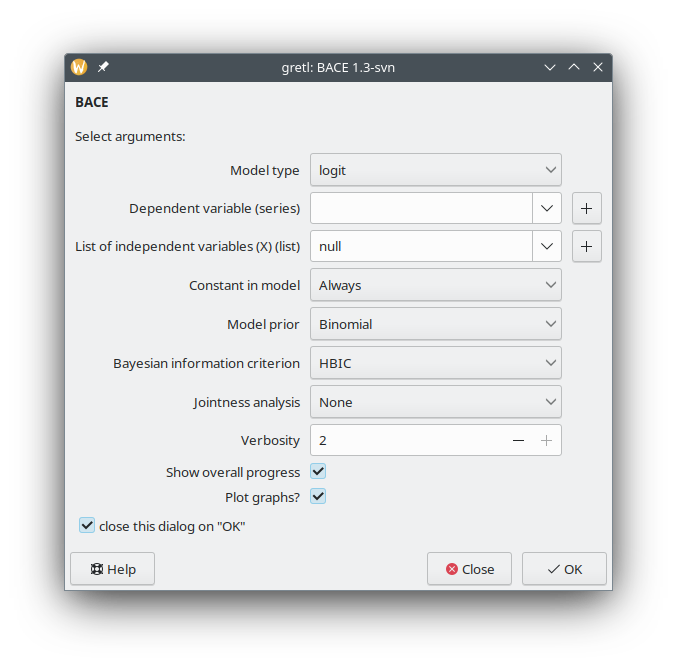
\includegraphics[width=0.7\columnwidth, keepaspectratio]{PNG/BACE_main_window}
	\caption{Main window for \cmd{BACE}.}
	\label{fig:Main window for BACE}
\end{figure}

According to Figure~\ref{fig:Main window for BACE}, we can specify the following
entries in the GUI \cmd{BACE} window\label{text:module_parameters}
\begin{itemize}
	\item \textbf{Model type} -- What kind of modeling should be
		should be performed?
	\item \textbf{Dependent variable} -- The dependent variable.
	\item \textbf{Y lags} -- number of lags for dependent variable
		(for time-series only).
	\item \textbf{List of independent variables}
		-- List of all independent variables (including lagged series).
	\item \textbf{Constant in model} -- Do we include intercept?
		It can be: always, never or can be dropped.
	\item \textbf{Bayesian information criterion} -- Version of BIC to
		be used.
	\item \textbf{Jointness analysis} -- If \cmd{None} (the default),
		the jointness analysis is omitted. Alternatively, one can
		choose one of the 7 available jointness measures.
	\item \textbf{Number of out-of-sample forecasts} -- Defines the
		total number of out-of-sample forecasts of the dependent variable.
	\item \textbf{Verbosity} -- An integer value of 1 or 2; the default
		is 2, so a more detailed description of the	analysis is provided
		(initial model, speed of convergence, estimation results for top
		ranked models).
	\item \textbf{Show overall progress} -- The progress bar is printed.
	\item \textbf{Plot graphs?} -- Shall we produce graphs?
\end{itemize}

\subsection{The script way}
\subsubsection{Script}
The \cmd{BACE} package can also be used inside \proglang{Hansl} scripts.
A very minimal code could be as follows:
%
\begin{lstlisting}
open greene9_1.gdt
include BACE.gfn

list greene = capital labor nfirm

BACE(valadd, greene)
\end{lstlisting}
The above code triggers BACE analysis with default option
described on page~\pageref{sec:default_option_bundle}.
On contrary, the corresponding ''big call'', i.e. with
setting all possible parameters, would be as follows:
\begin{lstlisting}
bundle opts = defbundle("model_prior", 2, "avg_model_size", 1.5, \
  "alpha", 0.6, "Nrank", 4, "do_joint", 0, "Npredict", 0, \
  "Nrep", 1000, "burn", 10, "verbosity", 2, "show_progress", 1, \
  "do_plot", 1, "model_type", "linear", "const_type", 1, \
  "bic_type", 1, "data_trans", 0)

BACE(valadd, greene, opts)
\end{lstlisting}

or alternatively with the new syntax for creating a bundle
on-the-fly:
\begin{lstlisting}
	BACE(valadd, greene, _(model_prior=2, avg_model_size=1.5, \
	alpha=0.6, Nrank=4, do_joint=0, Npredict=0, Nrep=1000, \
	burn=10, verbosity=2, show_progress=1, do_plot=1, \
	model_type="linear", const_type=1, bic_type=1, data_trans=0))
\end{lstlisting}
Since some parameters in option bundle are over-loadable,
the equivalent call looks like this:
\begin{lstlisting}
	BACE(valadd, greene, _(model_prior="beta-binomial", \
	avg_model_size=1.5, alpha=0.6, Nrank=4, do_joint="none", \
	Npredict=0, Nrep=1000, burn=10, verbosity=2, show_progress=1, \
	do_plot=1, model_type="linear", const_type="always", \
	bic_type="bic", data_trans="none"))
\end{lstlisting} 
The above example consists of three blocks.

\begin{lstlisting}
	open greene9_1.gdt
	include BACE.gfn
	set seed 1000000
	
	list greene = capital labor nfirm
	
	scalar model_type = 1
	scalar y_lags = 0
	scalar with_const = 1
	scalar data_trans = 0
	scalar model_prior = 1
	scalar bic_type = 1
	scalar hyperparameter = 0
	scalar prior_avg_model_size = 1.5
	scalar alpha = 0.6
	scalar top_ranked_model = 4
	scalar joint = 1
	scalar forecasts = 0
	scalar Nrep = 2000
	scalar Nburn = 10
	scalar verbosity = 1
	scalar progress = 1
	scalar plots = 1
	
	BACE_GUI(model_type, valadd, y_lags, greene, with_const,\
	data_trans, model_prior, bic_type, hyperparameter,\
	prior_avg_model_size, alpha, top_ranked_model, joint,\
	forecasts, Nrep, Nburn, verbosity, progress, plots)
\end{lstlisting}

The above example consists of three blocks.
The first block is just opening of the so called \cmd{greene9\_1}
dataset, which is bundled in every standard gretl installation.
This dataset contains cross-sectional data on manufacturing
of transportation equipment presented as Table 9.1 in
\cite{greene_Econometric_A}%
\footnote{This dataset is also available at link
	\url{http://people.stern.nyu.edu/wgreene/Text/Edition7/TableF7-2.txt}.}.
We also set the seed in order to exact reproduction of the results.

The second block is the definition of the \cmd{greene} list which
contains three independent variables available in the \cmd{greene9\_1} dataset.

The third block contains the definition for Bayesian Averaging of Classical
Estimates analysis: no lags for Y variable (not applicable since we have
cross-sectional data), constant always included, binomial model prior,
prior average model size set to 1.5 (which means that we have uniform model prior),
significance level for the initial model set to 0.6, 4 top ranked models,
jointness analysis with Ley-Steel Measure, without out-of-sample predictions,
10000 replications with 10\% burn-in draws, basic output (verbosity set to 1)
and progress overall progress is printed.

Suppose we want to run the same analysis but following
Occam's razor principle. The simplest way is setting the prior
average model size to 1. We also want to have ''random'' constant,
i.e. intercept can be dropped in any model. We also want to save
results of the BACE analysis in the bundle \cmd{results\_b},
the code should be as follows:
\begin{CodeChunk}
	\begin{CodeInput}
		prior_avg_model_size = 1
		with_const = 2
		
		results_b = BACE_GUI(valadd, y_lags, greene, with_const, model_prior, 
		prior_avg_model_size, alpha, top_ranked_model, joint, forecasts,
		Nrep, Nburn, verbosity, progress)
	\end{CodeInput}
\end{CodeChunk}

Suppose we want to calculate Doppelhofer-Weeks Measure instead of
already computed Ley-Steel Measure. Since the type of jointness measure
is controlled by \cmd{do\_join} field in the result bundle, the only thing
we have to do is to set the value of \cmd{do\_join} to 2 and print BACE
results again. The code should be as follows:
\begin{CodeChunk}
	\begin{CodeInput}
		results_b.do_joint = 2
		BACE_Print(&results_b)
	\end{CodeInput}
\end{CodeChunk}


\subsection{Output}\label{sec:outputs}
\textcolor{red}{\textbf{Outdated!!!}}\newline
If you select the appropriate entries in the GUI \cmd{BACE} window,
our package returns: Posterior Inclusion Probabilities (PIP), the
averages of the posterior means and standard deviations of parameters
(``Mean'' and ``Std.Dev.'', respectively) and the posterior mean and
standard deviation of each coefficient conditional on the variable
being included in the model (``Cond.Mean'' and
``Cond.Std.Dev.''). Furthermore, the package also returns the
predictive results for the dependent variable (``Mean'' and
``Std.Dev.'').

Let us consider the data used in previous example
(\cmd{australia.gdt}).  This dataset contains the Australian macro
data used in \cite{Johansen1995Likelihood} and originally supplied by
Tony Hall.  The variables used in the text are:
\begin{itemize}
	\item lpau -- log of Australian CPI (dependent variable),
	\item lpus -- log of US CPI,
	\item le -- log of exchange rate (price of US dollars in Aus. dollars),
	\item iau2 -- 5-year Treasury bond rate, Australia,
	\item ius2 -- 5-year Treasury bond rate, USA. 
\end{itemize}
Suppose we want to perform BACE analysis up to $ADL(2,2)$ specification,
i.e. all possible combinations from $ADL(0,0)$ to $ADL(2,2)$.
The example script would be as follows:

\begin{CodeChunk}
	\begin{CodeInput}
		set verbose off
		include BACE.gfn
		open australia.gdt
		genr time
		
		# We create lagged values
		adl_lags = 2
		lags(adl_lags, ius2)
		lags(adl_lags, iau2)
		lags(adl_lags, e2)
		lags(adl_lags, lpus)
		lags(adl_lags, le)
		
		# We define list with all X-es (including lags)
		list X_list = time ius2 ius2_* iau2 iau2_* e2 e2_* lpus lpus_* le le_*
		
		set seed 1000000
		scalar y_lags = 2
		scalar with_const = 2
		scalar model_prior = 1
		scalar prior_avg_model_size = (nelem(X_list) + y_lags + (with_const > 0)) / 2
		scalar alpha = 0.6
		scalar top_ranked_model = 4
		scalar joint = 0
		scalar forecasts = 4
		scalar Nrep = 20000
		scalar Nburn = 10
		scalar verbosity = 2
		scalar progress = 0
		
		RES = BACE_GUI(lpau, y_lags, X_list, with_const, model_prior, prior_avg_model_size,
		alpha, top_ranked_model, joint, forecasts, Nrep, Nburn, verbosity, progress)
	\end{CodeInput}
\end{CodeChunk}
In the above analysis all variables (including dependent variable $lpau_t$)
are lagged by 2 periods. Additionally we compute 4 forecasts:

\begin{CodeChunk}
	\begin{CodeOutput}
		Posterior moments (unconditional and conditional on inclusion):
		PIP         Mean     Std.Dev.    Cond.Mean Cond.Std.Dev
		lpau_1      1.000000     0.894595     0.091656     0.894595     0.091656
		ius2      0.996500    -0.418560     0.102196    -0.420030     0.099314
		lpus_2      0.790611    -0.303217     0.212152    -0.383523     0.161647
		lpus_1      0.780500     0.356760     0.260342     0.457092     0.202432
		iau2      0.752222     0.224487     0.161678     0.298432     0.112617
		le_2      0.506944    -0.027670     0.046149    -0.054582     0.052271
		const      0.392778    -0.074241     0.125663    -0.189015     0.136050
		e2_2      0.335667     0.002317     0.033496     0.006903     0.057540
		lpus      0.296222     0.037894     0.107134     0.127924     0.165014
		le_1      0.282500    -0.023085     0.062683    -0.081716     0.095485
		lpau_2      0.253056     0.037914     0.087083     0.149825     0.114894
		e2_1      0.245222     0.015275     0.052532     0.062292     0.091240
		time      0.233778     0.000053     0.000269     0.000226     0.000520
		iau2_1      0.231389     0.035210     0.090726     0.152166     0.133328
		le      0.211667     0.010063     0.042201     0.047542     0.081437
		e2      0.176222    -0.005057     0.034623    -0.028698     0.078258
		ius2_1      0.175222     0.021296     0.072659     0.121539     0.133961
		ius2_2      0.140111    -0.009023     0.048048    -0.064400     0.113626
		iau2_2      0.132000     0.005342     0.042150     0.040469     0.109717
		
		----------------------------------
		
		Posterior probability of models:
		Model 1:	0.024278
		Model 2:	0.020556
		Model 3:	0.012889
		Model 4:	0.009278
		Total probability of the models in ranking (numerical): 0.067000
		
		Correlation coefficient between the analytical
		and numerical probabilities of the above models: 0.932557
		
		----------------------------------
		
		Predictive results:
		lpau           Mean       Std.Dev.
		1990:2        5.334649       5.340552       0.007950
		1990:3        5.341856       5.356902       0.008400
		1990:4        5.368310       5.378660       0.010094
		1991:1        5.366443       5.395817       0.013705
	\end{CodeOutput}
\end{CodeChunk}

% The \cmd{BMA} estimate function accepts a scalar, which sets the verbosity
% of the output. Its default value is 1, which causes the estimation
% output to be printed out. A value of 2 forces the \cmd{BMA} function to
% print out all the details of the estimation. You can print out the
% above-mentioned results and additionally the following information:
% the total CPU time, type of model prior, prior average model size,
% significance level for the initial model, type of g-prior, total
% number of iterations and, finally, the number of burn-in
% draws. Moreover, the \cmd{BMA} estimate function produces the estimation
% results for the initial and top ranked models. The jointness analysis
% is inactive by default. If it is active, you will get: posterior joint
% probability of explanatory variables, jointness statistic as given in
% Equations~\ref{LS_jointness} or~\ref{DW_jointness} and classification
% of jointness measures.  The jointness analysis for the previous
% example should look like this:
% %
% \begin{CodeChunk}
	% \begin{CodeOutput}
		% Posterior joint probability of variables:
		%               GDPsh560 Confuncious   Life_Exp  Equip_Inv ...  
		%    GDPsh560   0.000000    0.889256   0.932182   0.903349 ...
		% Confuncious   0.000000    0.000000   0.826208   0.816956 ...
		%    Life_Exp   0.000000    0.000000   0.000000   0.839068 ...
		%   Equip_Inv   0.000000    0.000000   0.000000   0.000000 ...
		%         ...        ...         ...        ...        ... ...
		% Jointness statistics (Ley-Steel Measure):
		%               GDPsh560 Confuncious   Life_Exp  Equip_Inv ...
		%    GDPsh560   0.000000    2.083161   2.643181   2.235000 ...
		% Confuncious   0.000000    0.000000   1.576599   1.618373 ...
		%    Life_Exp   0.000000    0.000000   0.000000   1.662559 ...
		%   Equip_Inv   0.000000    0.000000   0.000000   0.000000 ...  
		%         ...        ...         ...        ...        ... ... 
		% Strong substitutes:
		%         Rev_Coup,Area       -4.516140
		% Rev_Coup,Publ_Edu_pct       -4.459739
		%                   ...             ...
		% Significant substitutes:   
		%        GDPsh560,Hindu       -1.997989
		%      Mining,War_Dummy       -1.989541
		%                   ...             ...   
		% Significant complements:
		%  Confuncious,Life_Exp        1.576599
		% Confuncious,Equip_Inv        1.618373
		%                   ...             ...
		% Strong complements:   
		%   DPsh560,Confuncious        2.083161
		%    GDPsh560,Equip_Inv        2.235000
		%                   ...             ...  
		% \end{CodeOutput}
	% \end{CodeChunk}
% %

%%% Local Variables:
%%% mode: latex
%%% TeX-master: "BACE_package_for_gretl"
%%% End:

%	\input{Empirical_illustration}
	
	\bibliographystyle{jae}
	\bibliography{BACE}
\end{document}

%%% Local Variables:
%%% mode: latex
%%% TeX-master: t
%%% End:
